\label{key}\documentclass[letterpaper, 12pt,oneside]{article}
\usepackage{amsmath}
\usepackage{graphicx}
\usepackage{xcolor}
\graphicspath{{Imagenes/}}
\usepackage[utf8]{inputenc}
\usepackage{listings}
\usepackage[hidelinks]{hyperref}

\title{\Huge Taller de Herramientas Computacionales}
\author{Josué Artemio Hernández Rodríguez}
\date{24/Enero/2019}

\begin{document}
	\maketitle
	\begin{center}
		
\includegraphics[scale=0.7]{3.jpg}
	\end{center}

	\newpage
	
	\title{\huge \textit{Bitacora problema 4 }}\\

	Este problema calcula el enésimo termino de la sucesión Fibonacci, le implemente una función llamada fib(n), y a partir de un caso base, que era n < 2, que me regresara el valor de n. pero si no, osea \textit{else} calculara la suma de fib(n-1) + fib(n-2), que son los dos anteriores, con una función recursiva. 
	
	 

	\begin{figure}[h]
		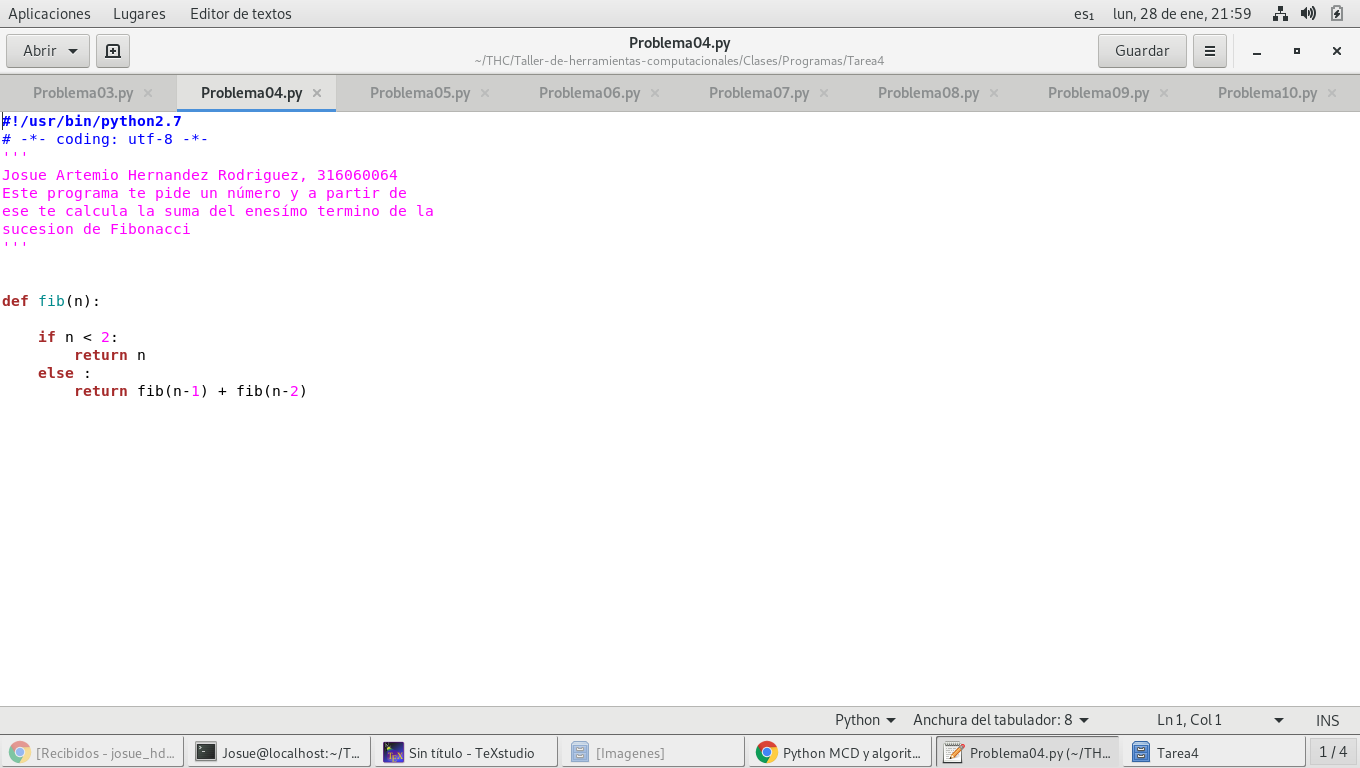
\includegraphics[scale=0.3]{pro04.png}
	\end{figure}
	
	
	
	
	
	
	
	
	
	
	
\end{document}
